\documentclass[12pt]{article}
\usepackage{float}
\usepackage{caption}
\usepackage{times}
\usepackage{natbib}
\usepackage{graphicx}
\usepackage[section]{placeins}
\usepackage{indentfirst}
\usepackage{fancyhdr}
\usepackage{xcolor}
\usepackage{enumitem}
\usepackage{listings}
\usepackage{color}
\usepackage[hyphens,spaces,obeyspaces]{url}
\usepackage{hyperref}
\pagenumbering{roman}
\usepackage{subfig}
\hypersetup{
    colorlinks=true,
    linkcolor=blue,
    urlcolor=blue,
    citecolor = gray,
    linktoc=all
}
\lstset { %
    language=C++,
    backgroundcolor=\color{black!5}, % set backgroundcolor
    basicstyle=\footnotesize,% basic font setting
}
\pagestyle{fancy}
\fancyhf{}
\rhead{\textit{\color{gray}\today}}
\lhead{\textit{\color{gray}C++14 Software Transactional Memory}}
\rfoot{Page \thepage}
\lfoot{\color{gray}\LaTeX}

\pagenumbering{roman}
\begin{document}

\begin{titlepage}
	\begin{center}
	\line(1,0){350}\\
	[0.3 cm]
	\huge{\textbf{Software Transactional Memory\\[0.3 cm]C++14 STM\\ }} 
	\line(1,0){200}\\
	[0.3 cm]
	\huge{\textbf{Final Report }} 
		\begin{LARGE}
		\\[0.3 cm]Zoltan Fuzesi\\
		\today
		\end{LARGE}
		
		\begin{LARGE}
		\line(1,0){150}\\
		[1.0 cm]
		Student ID: C00197361\\
		Supervisor: Joseph Kehoe\\
		\color{gray}Institute of Technology Carlow\\
		\color{gray}Software Engineering
		\end{LARGE}
		
\begin{figure}[h!]
\centering

\includegraphics[scale=0.7]{Pictures/carlow.png}

\end{figure}
		
	\end{center}
\end{titlepage}

\tableofcontents


\clearpage
\pagenumbering{arabic}
\setcounter{page}{1}
\section{Introduction}
This document summarizes all of the related works done, problems, errors, tests and learning outcomes, while developing Software Transactional Memory throughout the project lifetime. It will describing the library, the data structures and the related testing carried out.   

  
\section{About the project}
The purpose of this project to implement Software Transactional Memory, concurrency control solution as a Shared and Static library, that can be included in any C++ software application. Most of the STM (Software Transactional Memory) libraries works with a single primitive variable type, as it stores and protect the memory location of a single variable. Those type of STM solution doesn't need any extra implementation in order to use the library. This project produced a STM solution, that can store object instead of primitive variable memory location. Because the Shared or Static library able to take any type of object, and the library doesn't know anything about the client application objects, it uses polymorphic class hierarchy to achieve the required functionalities.\\

It's required extra implementation to the client application to inherit from the library base object. This inheritance gives a huge flexibility to my library to work with any type of unknown class instance. By the inheritance, the base object supports all the required fields and functions to the library, to carry out all the STM library (Software Transactional Memory) specific computations. To achieve Transactional Memory implementation, we can use programming language extensions, specific compiler support, that required to install or replace/upgrade the gcc/g++ complier on the developer system. My project not using this complier specific features, the logic was built from scratch, to implement the Software Transactional Memory implementation. I chose this way of implementation, because I want to learn as much as possible from this project and from the transactions.\\
 
With the previous testing and the short experience with the library, I can say the library can handle any number of threads with any number of objects. Of course, if we increasing the number of objects and the complexity of the transactions, the running time and the roll-back will significantly increasing. We can nesting our transactions to any level as we want, the library can handle it as well.\\

To use my STM library with any c++ application, we need to follows some rules to achieve the inheritance. The tutorials of this implementation and from the API functionality can be found on the project website.


\section{Problems encountered and resolved}
The most significant problem caused by the theory, such as use the library, with any c++ client application, as it store and modify the instances of any client application object within the transactions, without changing or customize the library code. To achieve this functionality it need a different way of thinking to developing the library. When the programmers building a new library for a given application, that compatible only with that application, and they can use a reference of all the client application classes in the library. It makes the development easier, but the code must be redesign/customize to every single application to work with.\\

The second biggest problem was to synchronize objects state with multiple threads, without using mutex lock in the code segments. Because, if we locking code segments, we narrowing down our application to sequential execution, where all transaction will be dependent on other transaction, however they are not using the same objects.\\

\textbf{These theoretical questions caused the following problems:}
\begin{enumerate}
\item Storing unknown objects. 
\item Template class and functions.
\item RAW pointers with polymorphic objects.
\item Segmentation fault.
\item Synchronizing load, store and commit functions without locking code segment.
\end{enumerate}
 
\subsection{Storing unknown objects}
During the research I have found the boost c++ library, as a best solution to store unknown objects. However, I didn't planned to use third party libraries, everywhere I have faced to the same answer. So, the boost library does the job, however in my solution without knowing the client application object to store it, the boost library doesn't helps at all. If I store primitive type rather than object type, the boost library could be a better solution. I tried to implement the solution, but it's required to use template class and functions, that caused the next problem. \textbf{\textit{3.2 Template class and function}}

\subsection{Template class and functions}
In c++ programming language, if we intend to use shared or static library with the client application, the header files must be include in the developed code directory/compilation process. If the code contains a template class or function, that means the code will be checked in runtime, and must be placed in the header file. So, if all the code relying on template class or function, the static or shared library can not be build, because only the *.cpp files are build into the library file. To solve this problem, I need to remove the boost library, and redesign the code with standard c++ solution, provided by the available libraries in the  language, and providing only the functions declaration in the c++ header files.

\subsection{RAW pointers with polymorphic objects}
During the research, all of the documentation found by the internet, was used RAW pointers. For this reason, and because the RAW pointers the fastest in c++ language, I used as a first solution. The RAW pointers did not cause any problem during the development, until the memory management test. The memory management test happened with \textbf{Valgrind} programming tool for memory debugging, memory leak detection, and code profiling. With this test in the project I have faced with memory leaks. The library use virtual method in the base class to copying the objects within the transactions, and these methods are implemented in the child classes, and can be used by the polymorphic class behaviour. This function cause memory leaks during copying the child class instance. I have tried to use smart pointer in this function to bridge the memory leaks, but because the library doesn't know anything about the connected classes, the casting in the library from smart pointer to RAW pointer is impossible without the target class reference.

\subsection{Segmentation fault, deadlock, live-lock}
This are the more frequent problems when working with multi threaded programming environment. Since the project not using mutex locks to lock code sections, apart from registering the the objects and transactions, it is a huge challenge to find where is the memory corruption deadlock or live-lock happens. Sometimes, the code executing correctly, but sometimes throws an error or just hanging forever, that depends the threads sequence execution in the background and the number of threads used in the process. The code might throws an error with hundred threads but might not if the process uses only ten threads. Even, if the code executing correctly, it should be executed multiple times, to make sure there is no corruption or other locking events happen.\\

I started to use the gdb default C++ debugger, but it is a bit difficult and time consuming when the process uses hundreds of threads. As a faster debugging solution I start printing out messages to the console from the different code segments, to narrowing down the error area, to the possible line of code segment where is the error raised by the thread.    

\subsection{Synchronizing commit function without locking code segment }
To synchronize the library commit function execution, the project use object base locking. If the code segment locked by a mutex lock, then all the transactions are dependent on the other transactions even if they are using different objects, and only one transaction can working at the same time. To solve the concurrent transactional execution, all the functions are completely lock free, and the transactions are locking the objects itself. This design blocking those transactions only, in which using any object that is participating in any another transactions. So, if we have five transactions, they are not using any object from another transaction, then all the transactions can make changes on their objects at the same time. 


\subsection{Resolved problems }

\subsubsection{Storing unknown objects }
To store unknown objects the project use inheritance/polymorphic behaviour as it stored the objects as a base class reference type. All the classes intend to use with the library, must inherit from the base class. If the project written in other programming language, we can argue about this solution, because might the language not supporting multiple inheritance, and the client application classes will be restricted to inherit from the base class only. Because, c++ programming language supporting multiple inheritance, then the client application classes are not restricted to achieve inheritance, polymorphic Object Oriented behaviour implementation from any other classes in the client application, but it gives me lots of freedom to control unknown objects in the library.

\subsubsection{Template class and function }
Because, the library store the unknown objects as a base class reference, there is no more required to use any template class or function in the library. All the code has moved into the cpp files, and only the class and function declaration left in the header files that is visible to the client application.

\subsubsection{RAW pointers with polymorphic objects}
The RAW pointers are replaced with smart pointer, that give me a freedom to use the polymorphic classes in the target class to copying the object from the external library. In this way the smart pointer get destroyed when goes out of the scope, and the memory leak has solved.

\subsubsection{Segmentation fault}
The segmentation fault was the most tricky part. If the application use for instance hundred transactions and six hundred objects, the possible permutations and combinations of the concurrent execution of transactions/threads are really big. If we running the same code twenty times might the code will faced with the segmentation fault if not well designed. Every time, when the code was changed, it was at least hundred times executed the same combination, to check the percentage of the code failure. During the development, the transactions was mixed up as complicated as possible, to try to causing segmentation fault early at code change. In this phase of the project life time, I have to say there was no segmentation fault in the last two iteration. But, because the possible complexity might can not be tested by one person, the segmentation fault might can be raised by other person who thinking a bit different way of the problem.\\   
   
\newpage
\section{Project description/achievement}
The initial goal was to implement a Software Transactional Solution in C++ language, where a piece of code executes a series of reads and writes to shared memory, and these logically occur at a single instant in time. The intermediate states should not be visible to other (successful) transactions.\\
\textbf{Mandatory}:
\begin{enumerate}
\item Full STM implementation. 
\item Full documentation of library with Doxygen.
\item Tutorial of library usage.
\end{enumerate}
\textbf{Discretionary}:
\begin{enumerate}
\item Library is tested across multiple platforms(Windows, Linux, MAC OSX). 
\item Website with downloadable libraries and demonstrate the usage.
\end{enumerate}
\textbf{Exceptional}:
\begin{enumerate}
\item Benchmarks: The library is fully benchmarked. 
\item Comparison: Compare with other STM approaches.
\end{enumerate}
\subsection{Achieved}
\textbf{Mandatory} : The STM implementation has achieved using any number of threads/transactions, and any number of objects/complexity. The prove that the transactions are not visible to other transactions, the test cases using multiple threads with the same objects, to cause race conditions. If the transactions are invisible to each other, and checking the other objects at commit time, the objects state should be consistent when all the transactions are finish with its changes on the objects.\\
The memory of course is shared between transaction, to prove it we can display the object values/state after all transactions finish with the computation on them, and if all the transactions accessed the same objects the final value/state should increased and consistent. To prove the STM not corrupting the objects within the transactions, we can execute the same code repeatedly, and the object state after the transactions finished should be same all the time.\\

The library fully documented with the Doxygen document generating tool and linked, available through the project website alongside the tutorials and the downloadable multi platform (Windows, Linux, MAC OSX) library files.\\

As an extra the transaction nesting is added to the library, where we can nesting our transactions to any level. It means, if the transaction dependent on other logical inner transaction, all the nested transaction will be executed as a a single unit.\\

\textbf{Discretionary} : The library is developed on the three main platform, Windows, MAC OSX and Linux. On Windows I used Visual Studio, because the MVSC (Microsoft Visual Studio Compiler) supporting the std::mutex that was used in the library, and the main c base language developer tool is the Visual Studio on Windows platform. On the Unix platforms, Linux and MAC OSX, I used Netbeans 8.2 as the development IDE. The main development and testing processes made on Linux system. The project website has tutorials to demonstrate the usage of the library.\\

\textbf{Exceptional}: Benchmarks, is not implemented yet, but hopefully it will be ready to the end of the project lifetime. To compare with other similar STM solution is not the easiest task, since my library using objects, and the most STM solution with available code using primitive type pointer based implementation. 

\subsection{Not achieved}
The Software Transactional Memory is a very research heavy area, and most of the papers I found during my research are from Master and PHD level. It is not an easy subject, and I should try using different data structure like binary tree, Red-Black tree, linked list and many other to compare the performance between them.\\


\newpage
\section{What learned}
During the development I have learning a lots from transactions, concurrency control and C++ language features.
\subsection{Technical learning}
\textbf{Transactions}:
\begin{enumerate}
\item What is transaction at all. 
\item How to implement atomic expression with my own code.
\item Have a fear idea how to implement transaction in any application in the future to protect shared memory space, where multiple user can access shared data with write access.
\end{enumerate}
\textbf{Concurrency control}:
\begin{enumerate}
\item Create lock free implementation of protecting critical section. 
\item Using object base locking, to prevent other threads to access same object at the same time.
\item How complicated can be working with multi threaded environment.
\end{enumerate}
\textbf{C++ language features}:
\begin{enumerate}
\item Difference between C++11, C++14, C++17.
\item Where to use RAW pointers and smart pointers.
\item Better knowledge/experience of C++ programming language.
\item Building code, using polymorphic programming features to handle unknown objects.
\end{enumerate}
\textbf{Static and Shared library implementation}:
\begin{enumerate}
\item Control the build of c++ programming language using Make file instead let the IDE to control the build process.
\item What is the difference between Static and Shared libraries.
\item Why is important to build libraries instead reuse, copy and paste the same code.
\end{enumerate}
\subsection{Personal learning}
\textbf{I have learned from my project:}
\begin{enumerate}
\item \textit{\textbf{Time management}}.\\
Deliver planned portion of the project for a given deadline. 
\item \textit{\textbf{Setting more specific targets for iterations}}.\\
There was no weakly plan for the iterations, I only had a big picture to achieve to the end of the iterations. 
\item \textit{\textbf{Why good research is very important.}}\\
If I spend a bit more time on a given question, that caused problem later in the development, that can save lots of time and I don't need to repeat a research around the given problem. 
\item \textit{\textbf{Design efficient code in productive way}}.\\
The first versions of the library contains huge amount code, where the single \textit{\textbf{load}} function was much bigger then the whole transaction class at the end of the project.
\item \textit{\textbf{Design the solution first in theory on paper, before jump into the code}}.\\
Before this project I had a bad hobbit, like jump into the code and design the the application on the fly. The structure of the project with the research and design documents shows a different way, how to think about the problem before start coding.     
\end{enumerate}

\section{What I would do differently if starting it again}
If I've to do this project again, I would spend bit more time with research on the object base locking and not spending that much time to find out all the compiler supported transactional syntaxes. My library use object rather than primitive type variable in the  library.\\

At the end my project ended up with object base locking and using the base operating system provided compiler. The area I would spend more time the pointers, and not relying on the opinion by other programmers and on my personal preference. If I use smart pointers from the begging, I don't need to redesign my code from RAW pointers to smart pointers.\\

The another area to spend more time is the way of store the unknown objects. When I found the third party boost library, I've finished the research and made my decision to use it. With a bit more research on boot library I could save lots of time, because most of the code needed to be redesign when it was replaced with standard map collection using inheritance. Otherwise, the project was out of my comfort zone, and everything about Software Transactional Memory concepts was completely new to me.\\

\section{Report on document update}
Between the design document and the final implementation there is some changes.
\begin{enumerate}
\item \textbf{There is no start transaction API function}.\\
The library API design was similar to TinyStm (STM library) API implementation, where is the client application need to notify the library to start the transaction. In my library solution, the singleton Transaction Manager manages all the transactions and the management is automatically behind the scene.  
\item \textbf{Object names and API function declarations}.\\
In the design document, perhaps in the first iterations the process id, and the thread id was part of the parameters in the API functions. Because, it makes the library usage very difficult, I tried to remove all the extra requirements in the API function parameters, and keep them as simple as possible. The object and function names are changed as well, now they are shorter and more meaningful.
\item \textbf{There is no functions to receive collections}.
In the design document I have separated functions to work with collections, but those ideas are removed from the final product. The client application can iterate through the collections to register and make changes on the objects. It gives full control on the objects to the client application rather than trusting in the library.
\item \textbf{Double version checking}.
The library use object based locking mechanism, that close out other transactions while a single transaction has ownership on the objects. With this design, the another transactions cannot access the same object and the double checking mechanism not necessary, only makes the execution time longer.
\item \textbf{Domain model}.
Actually the Domain model has change a lot about the API functions, for this reason I have added the new updated domain model to the Design Document with the connected sample classes. I found better way to manage the transactions, if I leave only few available options to the client application to use, and manage everything by the library automatically. In this way the library has less API function, that makes it easier to use, but has better management in my opinion. 
\end{enumerate}

\subsection{Additional research}
A small additional research required to the nested transactions implementation, because it was not in the description and the research was narrowed down to the main functionalities.\\
The another part that needed research, is unit testing for C++ programming language.\cite{cookbook} As everything else, the unit testing for c++ multi-threaded environment is more difficult then sequential programming.

\section{Module description}
The Software Transactional Memory C++ library, is a concurrency control mechanism, analogous to the database transactions. The library provide lock free programming solution to the client application, to manage shared memory spaces between transactions. The library built up from three main parts, Transaction Manager, the transaction object and the base object. If the client application using my library, then the way of programming in the client application is exactly same, as to programming a sequential coded application. The library take care of the thread synchronization, race-condition and memory corruption protection. The client application only need to create and use the threads, but doesn't need to worry about locking any function or code segment.   


\subsubsection{Transaction Manager}
The Transaction Manager responsible to manage all the transaction associated with the connected client application. When a Transaction Manager requested from the library, then a singleton object provided to the application to manage the transactional environment. The Transaction Manager is the only object who has permission to create a transaction object. The client application cannot create or request a transaction. This restriction was necessary to implement, because the library need full control on the created transactions with a single controller. Every single public API function in the library, could throw a runtime error, if the client application try to use an illegal or null pointer of an object.\\

\textbf{\textit{"TX EXIT"}} public function is providing the memory clearing management to the library. If the library shared, then the used memory by the main process should be cleaned up before the process exit. However, the library using smart pointer, that get destroyed when goes out of the scope, the process associated collections are still in the memory. The \textbf{\textit{"TX EXIT"}} function should be called by the client application, to delete all process maintained values. The Transaction Manager in this function deletes all the main process specific stored values, and calls the \textbf{\textit{"ostm exit"}} transactional function to clean up the global map from the main process specific memory spaces as well. In this way the shared library still running in the background in the operating system, but not accumulating the memory usage. \\ 


\begin{figure}[h!]
\centering
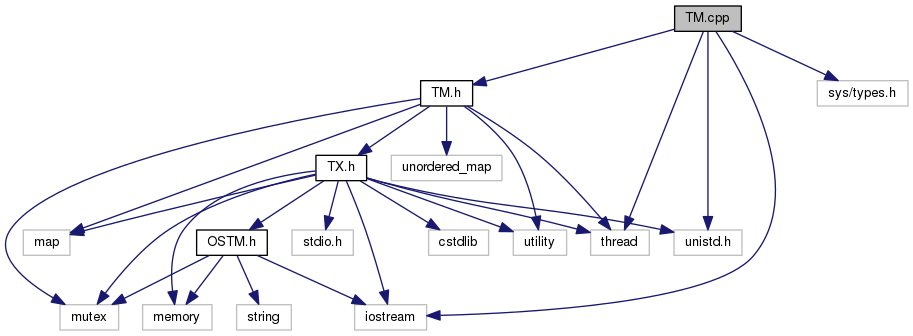
\includegraphics[scale=0.4]{Pictures/TM.png}
\caption*{\textit{\color{gray}Transaction Manager.}}
\end{figure}

\subsubsection{Transaction object}
The transaction objects created by the Transaction Manager can access the library API functions, to mange polymorphic objects throughout the transaction lifetime. It's including to register, load, store and commit the objects accessed by the transaction. There are more functions in the library, but those functions are not accessible to the client application. Those functions are private and automated within the transactions. Transaction can handle all process specific objects. The process can be the main process or light-weight process as well. To use transactions, doesn't need to used threads at all.\\

All transaction has private objects and collections, and sharing some class level field and collection too. The class level sharing necessary to use, because the library must let communicate the transactions when they needed. These communications are not controlled, since the thread sequence executions are completely random, controlled by the kernel. The communication happens in the register function, because all the transaction accessing the shared collection with write access. The sharing happens on the original objects between all the executing transactions when ever they needed, and its controlled by the objects locking mechanism itself.  



\begin{figure}[h!]
\centering
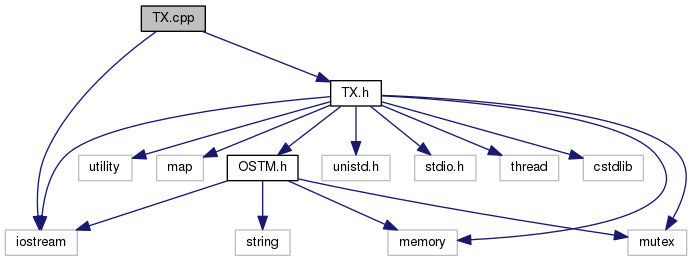
\includegraphics[scale=0.6]{Pictures/TX.png}
\caption*{\textit{\color{gray}Transaction Object.}}
\end{figure}

\subsubsection{Base object}
The base object provides all the required fields and functions to the inherited classes to work with the library. It is creating the uniqueness to the inherited objects, that required by the library to identify every single objects used, registered within the library. The base object providing the locking and the copying mechanism to the library as well, through polymorphic behaviour. 

\begin{figure}%
    \centering
    \subfloat[Inheritance from base object]{{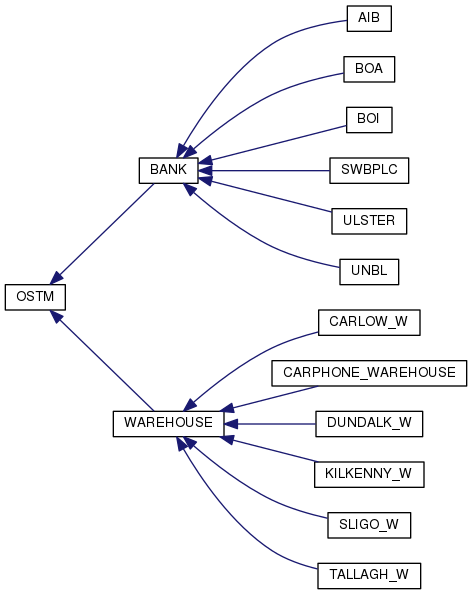
\includegraphics[width=6cm]{Pictures/BASE.png} }}%
    \qquad
    \subfloat[Target class inheritance]{{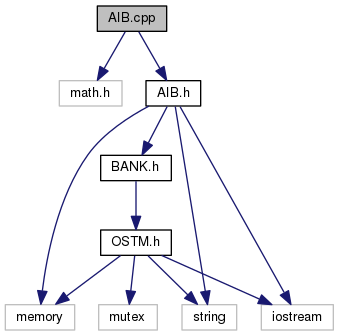
\includegraphics[width=6cm]{Pictures/aib.png} }}%
    \caption*{\textit{\color{gray}OSTM based object types}}%
    \label{fig:example}%
\end{figure}

\newpage
\subsection{Public API functions for transactions}
\subsubsection{Register}
The register function receiving a base class type smart pointer to register into the library. If the object already registered, the library will ignore the register request. When the object registered first time within the library, goes into the global shared map, and a copy of the object( working copy ) get registered in the transaction as well. This object will be used to make temporary changes associated with the target object, memory space during the transaction what is invisible to other transactions. 

\subsubsection{Load}
The client application can request for an temporary/working object using the original object reference. With this request the library returning the working object, to use by the client application. If the function receiving a illegal object, null pointer, or any object inherit from the base object, but not registered, that will throw a runtime error.

\subsubsection{Store}
When the client application wish to store the working copy of the object, it can use the store API function to save the changes during the transaction lifetime. If the object registered in the library, the object reference will update with the new changed object reference. If the function receiving a illegal object, null pointer, or any object inherit from the base object, but not registered, that will throw a runtime error.

\subsubsection{Commit}
The commit API call is the most complex function in the transaction. First the library need to check if the transaction is nested or not. If the transaction nested, then will call the private function to decrease the transaction associated value, and return to the client application to finish the outer transactions. If the transaction not nested, then need to find all the global shared object to lock them from the other transactions. If any of the transaction objects are locked in the global collection, then the transaction must wait in busy waiting, until the objects get unlocked buy the another transaction.\\

When the transaction get access/ownership to the object, then will lock it, and compare the version number associated with working copy and the original object. If any of the object within the transaction collection has different version number than the global shared original object, the transaction should finish and get the new updated values for all the working copies. When the transaction finishes, it will call the private function in the library, to unlock all the global objects associated with the transaction.\\

If the transaction committed all the changes on all the objects, then return true to the client application to indicate the transaction successful finished. If any version conflict was detected during the transaction, the function  returns false to the client application to indicate, it need to restart the transaction. Since, the commit function doesn't take any object reference, because it knows all the associated working copies and global shared objects with the transaction, we cannot cause any programmed error from outside in the commit phase with illegal object or null pointer.

\begin{figure}[h!]
\centering
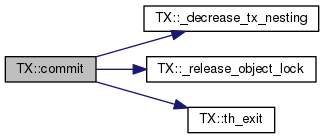
\includegraphics[width=6cm]{Pictures/commit.png}
\caption*{\textit{\color{gray}Automated functions.}}
\end{figure}

\subsection{Private API and Transaction Manager functions}
\subsubsection{Transaction Manager}
When the singleton Transaction Manager request for a transaction object, the transaction manager class checking the actual thread is registered in the manager or not. If the thread registered, the transaction associated with the thread is returned with increased the nesting counter. If the thread not registered, it will call the register private function, to register the thread in the manager. The register function including an another private function call, that returns a new map to store the thread within the manager.

\subsubsection{Transaction object}
During the register process, the transaction request a new map from a private function to every single application, to store all the associated transactions with the main process.\\
If the transaction finish or need to restart, will call the private function to release all the global shared objects, give access to the other transactions make changes on them.\\ 
When the transaction finish with the changes on the objects, it calls the exit private function to clean up all the associated working copies from the memory.\\

The transaction manger can  call a function to clean up the global shared map from all the associated memory spaces before the application exists.\\

The transaction manager can call a function to increase a value within the transaction to indicating the nesting level. To decrease a nesting level, the transaction need make a call from the commit function, if the transaction want to commit the changes, but the transaction is nested.

\section{Data structure}
There are many different collection type can be use to store the objects within the library. Actually, the collection type doesn't make different in the library functionality, but it can make different between the library performance. I have used the std::map, that is a sorted associative container, that contains key-value pairs with unique keys. I chose the map, because it has the fastest performance to access a unique object by the key in the collection without need to iterate through. However, the binary tree is a very fast data structure, but still needs to check the leaves from the root to find the requested object.\\

The library need to create good few collections to keep the association between processes and transaction.
\subsection{Transaction Manager}
To store all transactional objects created with Transaction Manager:
\begin{lstlisting}
std::map<std::thread::id, std::shared_ptr<TX>>txMap;
\end{lstlisting}
To store all process (threads) associated keys to find when deleting transactions. 
\begin{lstlisting}
std::map<int, std::map< std::thread::id, int >> process_map_collection;
\end{lstlisting}
Function used to return a map to insert to the process map collection as an inner value.
\begin{lstlisting}
std::map< std::thread::id, int > get_thread_Map();
\end{lstlisting}
\subsection{Transaction object (TX)}
To store parent based pointers to make invisible changes during isolated transaction.
\begin{lstlisting}
std::map< int, std::shared_ptr<OSTM>  > working_Map_collection;
\end{lstlisting}
To store parent based pointers to control/lock and compare objects version number within transactions.
\begin{lstlisting}
std::map<int, std::shared_ptr<OSTM>  >main_Process_Map_collection
\end{lstlisting}
To store all process associated keys to find when deleting transactions.
\begin{lstlisting}
std::map<int, std::map< int, int >> process_map_collection;
\end{lstlisting}
Function used to returning and map to insert to the process map collection as an inner value
\begin{lstlisting}
std::map< int , int > get_thread_Map()
\end{lstlisting}
\section{Testing}
As part of the developer tools I used CppUnit, unit testing framework to test the API functions and the library functionality.  
\textit{CppUnit is the C++ port of the famous JUnit framework for unit testing}.\cite{sourceforge}\cite{cookbook}. I have described few testing methods in the Design Manual document to prove the library correct functionality. All those testing methods are implemented, but because those methods are not so advanced testing perspectives, I added more complex test to prove that it works as it suppose to.\\
\textbf{Main tests}:
\begin{enumerate}
\item Multi threaded multiple object exchange test.
\item Multi-threaded single Object test.
\item Single-threaded multiple object test.
\item Multi-threaded multiple Objects test.
\item Testing the API store, load and register functions.
\item Complex transaction with multiple threads and object collections.
\end{enumerate}

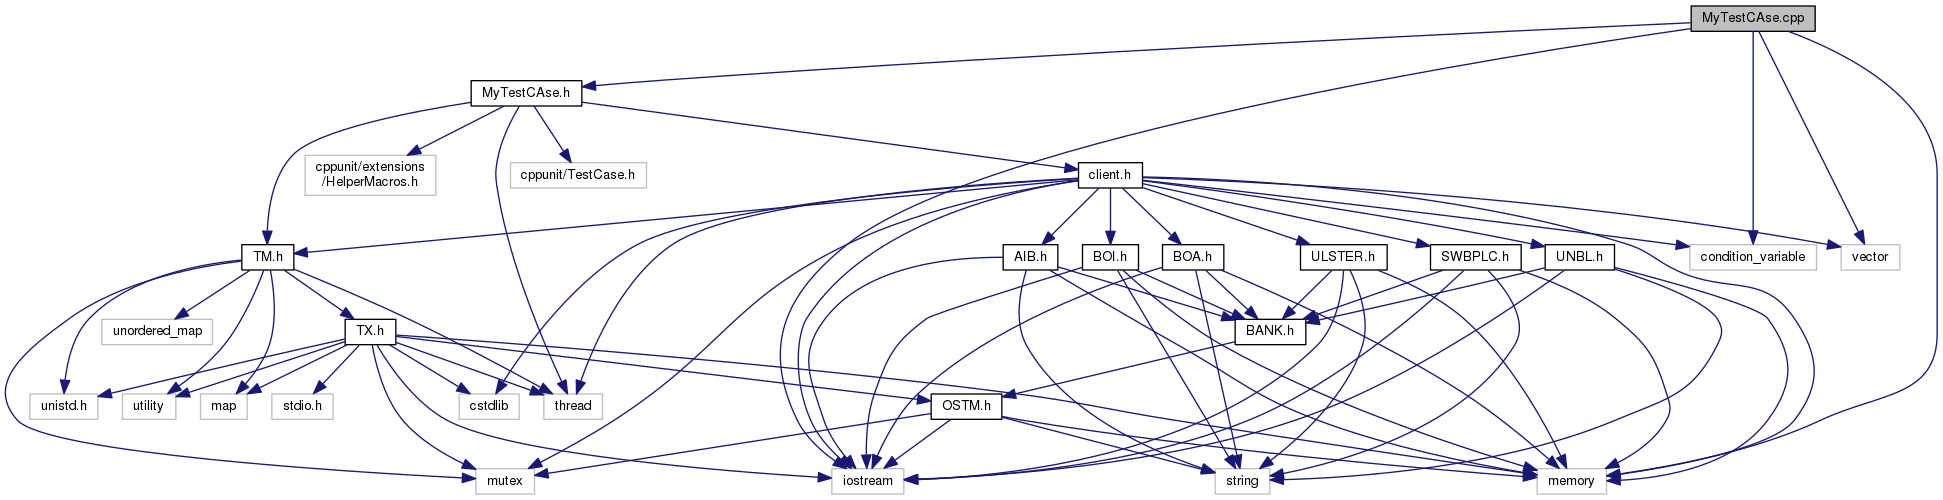
\includegraphics[scale=0.2]{Pictures/test.png}

\textit{\textbf{The documentation with the test code from the CppUnit test, can be found on the project website under CppUnit test.}}
\section{Conclusion}
This project was out of my comfort zone, with the concurrent programming and the Transactional environment. During my internship I have met with the transactions in Java framework, and now I had chance to learn how to implement it in C++ programming language. This project is really different from another project or from previous experience, where we need to create communication between programming components, create GIU interface to interact with the system and store values in the database.\\

This project required to produce a library(s), that can be used by other ++ applications. The most time consuming part of the project was to find out the best base class and create the client application to use the library, with the polymorphic objects/classes, that is after all not part of the final product, but without that development and implementation the library development is impossible to carry out.\\

I think it is not an easy subject, since we need to working with multi threaded environment, without any visual feedback. The only visual feedback is the console could be, where is the threads can printing out the feedback/string in any order, since we are not using lock in the code segment. If we using lock in the code segment to control the threads visual feedback, then the code is behaving differently then it suppose to be.\\ 

I have learned a lot from this project, how to control multiple threads without locking, and implement transactional environment without using any framework or someone else library. However, Software transactional Memory obsolete over the past few years, I think it is a very good experience/knowledge to know how transactions are implemented in the applications or libraries.
\newpage
\section{Bibliography}
\begin{center}
\bibliographystyle{abbrv}
\bibliography{database.bib}

\end{center}


\end{document}
